% Chapter 9 -- Claim: Momentum Works
% Requires: amsmath, amssymb, booktabs, array, tabularx, graphicx, tcolorbox (breakable, skins), hyperref or url.
% Defines the callout box only if the preamble has not.
\providecolor{fenavy}{HTML}{1B2A6B}
\providecolor{feshade}{HTML}{F3F5FA}
\makeatletter
\@ifundefined{callout}{%
  \newtcolorbox{callout}{breakable, enhanced,
    colback=white, colframe=gray!70, boxrule=0.5pt, arc=1mm,
    borderline west={2.5pt}{0pt}{gray!70},
    left=8pt, right=8pt, top=4pt, bottom=4pt}%
}{}
\makeatother

\chapter{Claim: Momentum Works}
\label{ch:09}

If value says buy what is cheap, momentum says buy what has been going up. Stocks that have outperformed over the past year tend to keep outperforming for months afterward, and stocks that have lagged tend to keep lagging. Stated so plainly, the idea sounds like a chart-reader's superstition, and for decades efficient-markets economists treated it as one. Yet momentum has become one of the most thoroughly documented patterns in finance, found in a century of U.S. data, in dozens of countries and in asset classes from bonds to commodities.

Momentum also has a dark side that the average return conceals. Every so often it loses, in a few months, much of what it gained over years. Those crashes are not random: they cluster at moments that can be described in advance, when a falling market suddenly turns.

This chapter puts the claim on trial and asks two questions an investor needs answered: does the premium survive scrutiny, and can its crashes be managed well enough for anyone to hold it?

By the end of the chapter you will be able to:

\begin{itemize}
  \item compute the standard 12--1 momentum signal and explain why it skips the most recent month;
  \item distinguish cross-sectional from time-series momentum;
  \item scale a position to a volatility target using only past data;
  \item explain underreaction and overreaction, and how a long--short portfolio's beta changes over time;
  \item state the claim that momentum works in a form that can fail, and test it over time, across markets, after costs and through its crashes;
  \item explain why momentum crashes after market rebounds, and how volatility scaling manages that risk.
\end{itemize}

\section{Foundations: past returns, two kinds of momentum, and investor behavior}
\label{sec:09-foundations}

\textbf{Measuring past performance.} A stock's past return over a window is its cumulative return over those months: $(1 + R_1)(1 + R_2)\cdots(1 + R_k) - 1$. The standard momentum signal uses the return from twelve months ago to two months ago, written ``12--1'' or ``12--2'': it covers eleven months and \textbf{skips the most recent month} (Figure~\ref{fig:09-signal}). The skip exists because returns over a single month tend to reverse (Chapter 6's short-term reversal); including that month would mix two opposite effects.

\begin{figure}[htbp]
\centering
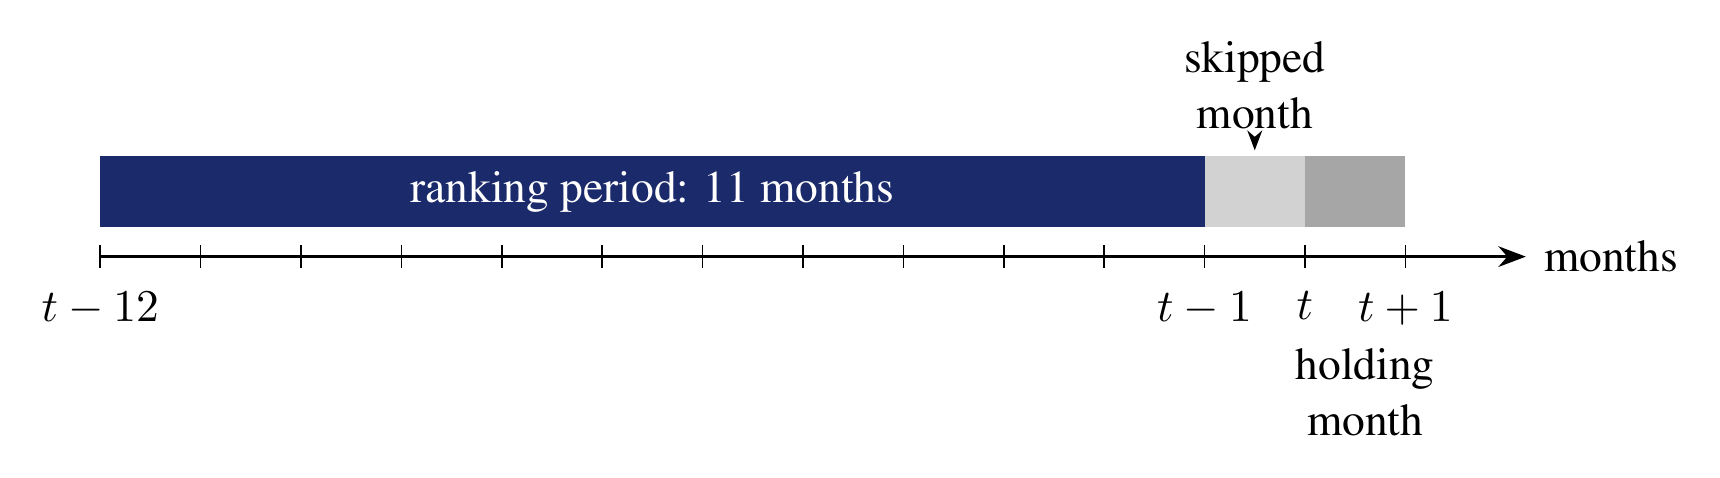
\includegraphics[width=0.9\linewidth]{images/fig09-1-signal.png}
\caption{The 12--1 momentum signal. Stocks are ranked on their return over the eleven months from $t-12$ to $t-1$; the most recent month is skipped; the portfolio is held for the month that follows.}
\label{fig:09-signal}
\end{figure}

\textbf{Cross-sectional momentum.} \textbf{Cross-sectional} or \textbf{relative} momentum ranks stocks against each other: buy the stocks with the highest past returns (\textbf{winners}) and sell those with the lowest (\textbf{losers}), regardless of whether the market as a whole rose or fell. Its long--short portfolio is \textbf{market-neutral} on average: over time its beta to the market is close to zero. The Fama--French momentum factor, often called \textbf{UMD} (up minus down) or Mom, is built this way, from six portfolios sorted on size and past return, in the same style as HML (Section~\ref{sec:08-how}).

\textbf{Time-series momentum.} \textbf{Time-series} or \textbf{absolute} momentum looks at each asset on its own: hold it long if its own past return is positive, short if negative. It is also called \textbf{trend following}, and it is what most \textbf{managed-futures funds}, funds that trade futures contracts across many markets, do. Unlike cross-sectional momentum it can be \textbf{net long} or \textbf{net short} the market, holding more long than short positions or the reverse, and it is usually applied across asset classes: stock indices, government bonds, currencies and commodities.

\textbf{Volatility scaling.} Many strategies size positions inversely to recent volatility, holding more when markets are calm and less when they are turbulent. If a position is scaled to
\begin{equation}
  w = \frac{\sigma^*}{\hat\sigma}
  \label{eq:09-volscale}
\end{equation}
where $\sigma^*$ is a target volatility and $\hat\sigma$ a forecast of the asset's volatility, its risk stays roughly constant over time. With a 12\% target and a forecast of 24\%, the position is halved; with a forecast of 8\%, it is one and a half times the base size. The forecast must use only data available before the position is set.

\textbf{Underreaction and overreaction.} \textbf{Behavioral finance} studies how investors' systematic errors affect prices. Two errors matter here.

\begin{itemize}
  \item \textbf{Underreaction}: investors adjust too slowly to news, because of conservatism or limited attention, so prices drift in the direction of the news for months.
  \item \textbf{Overreaction}: investors extrapolate a run of good or bad news too far, pushing prices past their fair value, which later reverses.
\end{itemize}

Momentum at horizons of a few months to a year fits underreaction or delayed overreaction; the long-run reversals documented by De Bondt and Thaler (1985) fit overreaction followed by correction.

\textbf{Beta that changes over time.} A long--short portfolio's market beta is the beta of its long side minus the beta of its short side. When the composition of the portfolio changes, so does its beta. After a market crash, the stocks that fell most, the losers, are typically high-beta stocks, so a momentum portfolio that is short them has a large negative beta. If the market then rebounds sharply, the portfolio loses heavily. This simple mechanism, explained in Section~\ref{sec:09-how}, accounts for momentum's worst months.

\textbf{Worked example.} A stock returned +40\% from twelve months ago to two months ago and $-5$\% last month. Its 12--1 momentum signal is +40\%, ignoring last month. If it ranks in the top 30\% of stocks on that signal, the momentum factor holds it in the winner portfolio for the coming month.

\textbf{Further reading.} Bodie, Kane and Marcus, \emph{Investments}, chapters on market efficiency and behavioral finance; Ilmanen, \emph{Expected Returns}, chapters on momentum and trend following; Ang, \emph{Asset Management}, chapter on factor strategies.

\section{How it works}
\label{sec:09-how}

\textbf{The strategy.} At the end of each month, rank stocks on their 12--1 past return. Buy the top group, sell the bottom group, hold for a month, and repeat. Because the ranking window shifts by one month at a time, ten of its eleven months carry over, and about a third of each side of the portfolio is replaced each month (Chapter 6). Jegadeesh and Titman (1993) studied many combinations of ranking and holding periods from three to twelve months; the 12--1 ranking with a one-month hold has become the standard.

\textbf{Why momentum might exist.} Three families of explanation compete.

\begin{itemize}
  \item \textbf{Underreaction.} Investors update slowly. Good news about a firm is only partly reflected in its price at first, and the rest arrives over the following months. Hong and Stein (1999) model news diffusing gradually through the investor population; Barberis, Shleifer and Vishny (1998) model investors who are too conservative in updating their beliefs.
  \item \textbf{Delayed overreaction.} Daniel, Hirshleifer and Subrahmanyam (1998) argue that overconfident investors, seeing their views confirmed by early price moves, push prices further than fundamentals justify, producing momentum in the medium term and reversal later.
  \item \textbf{Risk.} Momentum's crashes are themselves a candidate explanation: a strategy that loses heavily in rare, sharp market rebounds may earn a premium for bearing that risk. Rational models in which expected returns vary with firms' growth options have also been proposed, though none has become standard.
\end{itemize}

\textbf{Crashes and changing beta.} Momentum's market beta is not constant (Figure~\ref{fig:09-beta}). In a rising market, past winners are high-beta stocks and momentum has positive beta. After a market decline, past losers are the high-beta stocks and momentum is short them, giving it a strongly negative beta. Grundy and Martin (2001) noted this time variation; Daniel and Moskowitz (2016) showed that it explains momentum's crashes, which occur when markets rebound after a decline, and that their timing is partly predictable from the past market return and recent volatility.

\begin{figure}[htbp]
\centering
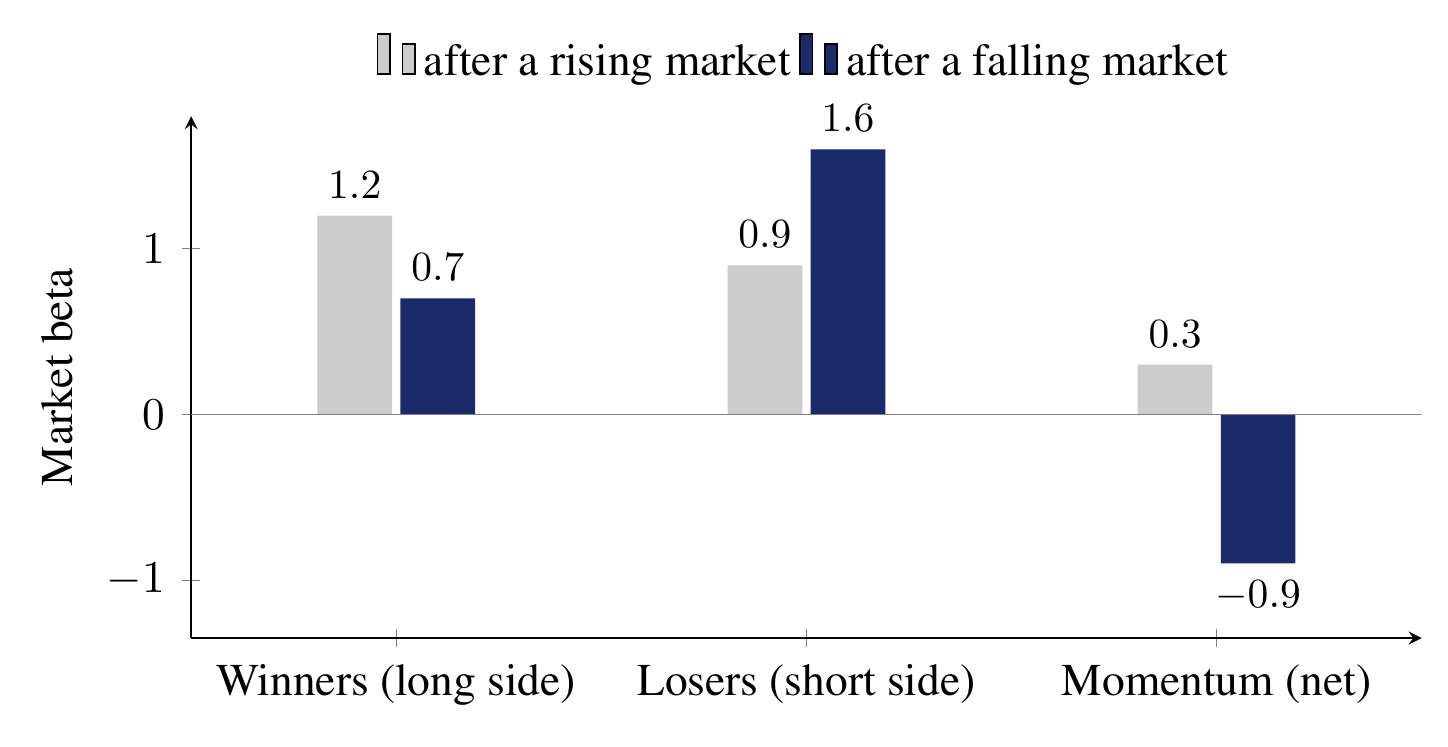
\includegraphics[width=0.85\linewidth]{images/fig09-2-beta.png}
\caption{Why momentum's beta flips (illustrative values). After a rising market the winners it holds are the high-beta stocks, so its net beta is positive. After a falling market the losers it sells short are the high-beta stocks, so its net beta turns strongly negative, and a sharp market rebound produces a large loss.}
\label{fig:09-beta}
\end{figure}

\textbf{Managing the crashes.} Because momentum's volatility rises sharply before and during crashes, scaling the position by forecast volatility, as in Equation~\eqref{eq:09-volscale}, cuts exposure when crashes are most likely. Barroso and Santa-Clara (2015) found that this nearly doubled momentum's Sharpe ratio and largely eliminated its crashes in U.S. data. Daniel and Moskowitz (2016) proposed a dynamic version that also uses a forecast of momentum's mean return.

\section{The claim}
\label{sec:09-claim}

Stated so that it can fail:

\begin{callout}
\textbf{Stocks with high returns over the past year continue to outperform stocks with low past returns over the following months, by enough to survive costs, in data beyond the samples that established the result, and with risks an investor can manage.}
\end{callout}

The final clause is what distinguishes this chapter's claim from a simple statement about average returns. A premium that is real on average but delivers losses of 50\% or more in a few months may be a premium few investors can collect. The tests follow:

\begin{itemize}
  \item \textbf{Time.} Is the premium present after Jegadeesh and Titman's 1965--1989 sample, and in every era?
  \item \textbf{Breadth.} Is it found in other countries and asset classes?
  \item \textbf{Costs.} Momentum trades far more than value. Does its premium exceed its costs?
  \item \textbf{Crashes.} How large are the crashes, can they be anticipated, and does managing them change the verdict?
\end{itemize}

\section{The original evidence}
\label{sec:09-evidence}

\textbf{Jegadeesh and Titman (1993)} sorted U.S. stocks from 1965 to 1989 on their past three- to twelve-month returns and found that buying winners and selling losers earned about 1\% a month, a result that could not be explained by market risk. They also found that part of the profit reversed after a year or more. \textbf{Jegadeesh and Titman (2001)} returned to the question with the years after their first paper and found that momentum continued to earn a similar premium out of sample, one of the earliest successful post-publication tests of an anomaly.

\textbf{Carhart (1997)} added a momentum factor to the Fama--French three-factor model to study mutual fund performance. The four-factor model became a standard benchmark, and Carhart's finding that much of the apparent persistence in fund returns was momentum exposure rather than skill was influential in its own right. Fama and French themselves did not include momentum in their models, while noting that their three factors could not explain it.

\textbf{Breadth.} Rouwenhorst (1998) found momentum in twelve European markets. Asness, Moskowitz and Pedersen (2013) found it in stocks across countries and in government bonds, currencies and commodity futures. Moskowitz, Ooi and Pedersen (2012) documented \textbf{time-series momentum} in 58 futures and forward contracts across four asset classes: an asset's own past twelve-month return predicted its return over the next month in almost every market studied. The notable exception is Japan, where Chui, Titman and Wei (2010) and others found cross-sectional momentum weak or absent.

\textbf{Crashes.} Daniel and Moskowitz (2016) documented that momentum's worst losses come in clusters after market declines, when the market rebounds. In the spring of 2009, as the market recovered from the financial crisis, past losers, many of them battered financial and cyclical stocks, rose far more than past winners. A similar episode occurred in 1932. The crashes were large enough that momentum's long-run return, though positive, came with negative skewness and extreme drawdowns. Barroso and Santa-Clara (2015) showed that scaling by forecast volatility removed much of this risk in U.S. data.

\section{Replication lab: Lab 9}
\label{sec:09-lab}

\begin{callout}
\textbf{Lab 9 at a glance.} \emph{The question:} has momentum earned a premium throughout the century of U.S. data, when do its crashes occur, and can volatility scaling make it a strategy an investor could hold? \emph{Data:} Kenneth French's library: the monthly and daily momentum factor from the 1920s, the market factor and risk-free rate, ten portfolios sorted on 12--2 past returns, and ten industry portfolios. Optionally, the Jensen--Kelly--Pedersen data for momentum in many countries. \emph{Code:} repository folder \texttt{ch09-momentum/}, with a guided notebook.
\end{callout}

\textbf{The setup.}

\begin{itemize}
  \item \textbf{Part A, replication.} Momentum's average return, t-statistic, Sharpe ratio, skewness, worst month and \textbf{maximum drawdown}, the largest fall from a previous peak, over the full sample, by decade, before and during the Jegadeesh--Titman sample, and after publication. The average returns of the ten momentum deciles show whether returns rise steadily from losers to winners.
  \item \textbf{Part B, crashes.} The ten worst months, with the market's return that month and over the previous two years. A regression of momentum on the market, with extra terms for \textbf{bear markets} (here, periods when the market's past 24-month return is negative) and for bear-market months in which the market rises, measures how momentum's beta changes.
  \item \textbf{Part C, volatility scaling.} Each month, momentum is scaled to a 12\% annual volatility target using the volatility of its daily returns over the previous six months. Its results are compared with raw momentum levered to the same average volatility, so the comparison is about timing, not leverage.
  \item \textbf{Part D, time-series momentum.} Each of ten industry portfolios and the market is held long or short according to the sign of its past twelve-month excess return, scaled to equal volatility. This is a narrow, equity-only version of Moskowitz, Ooi and Pedersen's test, and the lab says so.
  \item \textbf{Part E, costs.} Net returns at one-way costs of 20 and 50 basis points, using momentum's turnover of about 35\% a month.
\end{itemize}

\textbf{What readers will find.} Figure 9.3 marks the five worst months on a century-long chart of momentum's growth; Figure 9.5 shows that they cluster in the upper right of a scatter of momentum against the market during bear markets: when beaten-down markets rebound. Figure 9.6 compares raw and volatility-scaled momentum, with their drawdowns. The test of the claim is whether the premium is present in most decades and after publication, survives costs, and whether its crashes are manageable without hindsight.

\section{Stress tests}
\label{sec:09-stress}

\textbf{1. After publication.} Jegadeesh and Titman's paper appeared in 1993. Momentum's post-publication record is one of the longest out-of-sample tests of any anomaly, and Jegadeesh and Titman (2001) found it continued to work through the 1990s. The lab extends the test to the present, through the 2009 crash and the 2010s.

\textbf{2. Other countries and asset classes.} The international evidence is broad but not universal: momentum is strong in Europe and weak in Japan. The JKP data allow a country-by-country count, with Chapter 4's caution about how many significant results to expect by chance.

\textbf{3. Costs.} With turnover of about 35\% a month on each side, momentum pays four times that fraction of the one-way cost each month (Equation~\eqref{eq:06-net}). At 20 basis points, costs absorb roughly $4 \times 0.35 \times 0.20 \times 12 \approx 3$ percentage points of the annual premium; at 50 basis points, about 8. Novy-Marx and Velikov (2016) estimated momentum's costs at about 0.65\% a month and found it still earned a significant net premium, unlike higher-turnover strategies (Chapter 6). Volatility scaling adds trading when the weight changes; the lab charges for that too.

\textbf{4. Crashes and their predictability.} A crash that could be predicted only with hindsight is no help to an investor. The lab uses only information available at the start of each month: the past 24-month market return for the bear-market indicator, and past daily volatility for scaling. The test is whether those signals, set in advance, reduce the crashes.

\textbf{5. The volatility-scaling result itself.} A result that improves on a famous anomaly by adjusting it is itself a claim that can be overfit. Barroso and Santa-Clara chose a six-month window and a 12\% target; the lab lets readers change both, and an exercise asks how sensitive the improvement is. Chapter 11 returns to whether volatility timing works in general.

\section{Verdict}
\label{sec:09-verdict}

Based on the published evidence, to be confirmed by readers' runs of Lab 9 on data through 2025: \textbf{survives, with severe crash risk.}

\begin{center}
\small
\begin{tabularx}{0.9\linewidth}{@{}>{\raggedright\arraybackslash}p{0.22\linewidth}>{\raggedright\arraybackslash}X>{\raggedright\arraybackslash}p{0.25\linewidth}@{}}
\toprule
Test & Finding & Effect on the claim \\
\midrule
A century of U.S. data & A large average premium with a high t-statistic & Supports \\
After publication & Continued to earn a premium through the 1990s; weaker and more volatile since 2000, with the 2009 crash & Supports, weakened \\
Other countries and assets & Broad, with Japan the notable exception & Supports \\
Costs & Large, but smaller than the gross premium at institutional costs & Supports, with a smaller net premium \\
Crashes & Rare, severe and concentrated in market rebounds after declines & A serious qualification \\
Volatility scaling & Reduces crashes and raises the Sharpe ratio in the literature, using only past data & Supports manageability, but is itself a claim to test \\
\bottomrule
\end{tabularx}
\end{center}

Momentum is among the most robust anomalies in finance: it has survived publication, appears in most markets and asset classes, and covers its costs at institutional trading costs. Its crashes are the reason the verdict is not an unqualified survives: an investor holding raw momentum must be prepared to lose a large fraction of the strategy's value in a few months, at moments when the rest of the portfolio is recovering. The verdict is dated by the sample tested.

\section{What investors can use}
\label{sec:09-investors}

\textbf{Trend rules for asset allocation.} Time-series momentum applied across asset classes, the core of managed-futures funds, has historically tended to do well in prolonged market declines, when it turns short. That makes it a candidate \textbf{diversifier}, an addition that tends to do well when the rest of the portfolio does badly, for a stock-heavy portfolio. Its returns have been uneven, with long flat periods, and its fees are often high.

\textbf{Stock-picking momentum.} Cross-sectional momentum is best held as one component of a multi-factor portfolio. It is negatively correlated with value, so combining the two smooths returns (Asness, Moskowitz and Pedersen 2013). On its own, its crashes make it hard to hold.

\textbf{Manage the risk, not just the return.} Volatility scaling, or at least sizing a momentum allocation so that a 50\% loss in a few months would be survivable, is more important than any refinement of the signal.

\textbf{Questions to ask a momentum or trend-following manager:}

\begin{enumerate}
  \item How did the strategy perform from March to May 2009, and what would it do in a similar rebound?
  \item Is the position sized by volatility, and was that rule fixed before the backtest?
  \item What is the strategy's turnover, and what costs were assumed? How do they compare with your live trading costs?
  \item How much of the return comes from small, illiquid stocks?
  \item Over which periods has the strategy failed to make money, and for how long?
\end{enumerate}

\begin{callout}
\textbf{What Failed: holding raw momentum through the 2009 rebound.} By early 2009 momentum had performed well through the financial crisis: it was long defensive winners and short the collapsing financial and cyclical stocks. When the market turned in March 2009, the most beaten-down stocks rebounded hardest. Over the following months, momentum's loser portfolio rose far more than its winner portfolio, and the strategy lost much of a decade's gains in a few months (Daniel and Moskowitz 2016). Nothing about the crash was a mystery afterward: the strategy was short a portfolio of very high-beta stocks at the bottom of a bear market. The failure was in treating momentum's average return as the whole story, and in sizing positions as if the risk were constant. The claim that momentum's historical return could be harvested without managing its crash risk \textbf{fails}.
\end{callout}

\section{Open questions}
\label{sec:09-open}

\begin{itemize}
  \item \textbf{Can momentum crashes be forecast in real time?} The bear-market and volatility signals help in sample. How well do they work for an investor who adopts them today, and do they survive Chapter 4's multiple-testing corrections?
  \item \textbf{Why not Japan?} Cultural explanations, differences in investor behavior and differences in market structure have all been proposed for momentum's weakness in Japan; none is settled.
  \item \textbf{Risk or behavior?} If crashes are the risk that momentum's premium compensates, managing the crashes should reduce the premium. Does it?
  \item \textbf{Momentum in factors.} Ehsani and Linnainmaa (2022) argue that factor returns themselves have momentum. How does that relate to momentum in individual stocks?
\end{itemize}

\section*{Exercises}
\addcontentsline{toc}{section}{Exercises}

\subsection*{Conceptual (all readers)}

\begin{enumerate}
  \item Why does the standard momentum signal skip the most recent month? What would happen to the strategy's returns if it did not?
  \item Explain the difference between cross-sectional and time-series momentum. In a year when every stock rises, what does each strategy do?
  \item Explain, using betas, why momentum loses when a falling market rebounds sharply.
  \item Volatility scaling raised momentum's Sharpe ratio in the original study. List two reasons the improvement might be smaller for an investor who adopts it now.
\end{enumerate}

\subsection*{Lab extensions (technical readers)}

\begin{enumerate}
  \setcounter{enumi}{4}
  \item Re-run Part C with a weight cap of 1.5 and with targets of 8\% and 16\%. How sensitive is the improvement?
  \item Replace the 24-month bear-market indicator with a 12-month one. Does the crash regression change?
  \item Compute momentum's net Sharpe ratio after 2001 with a one-way cost of 10 basis points. Is momentum more implementable today?
  \item In Part D, change the look-back from 12 months to 3 and to 24. How does time-series momentum change?
  \item Using the JKP data, count the countries in which momentum has a t-statistic above 2. How many would you expect by chance?
  \item Combine momentum and value (Chapter 8) in a 50/50 portfolio. Compare its Sharpe ratio, skewness and worst drawdown with each strategy alone.
\end{enumerate}

\section*{References}
\addcontentsline{toc}{section}{References}

\begin{itemize}
  \item Asness, C. S., Moskowitz, T. J. and Pedersen, L. H. (2013). Value and Momentum Everywhere. \emph{Journal of Finance} 68(3): 929--985.
  \item Barberis, N., Shleifer, A. and Vishny, R. (1998). A Model of Investor Sentiment. \emph{Journal of Financial Economics} 49(3): 307--343.
  \item Barroso, P. and Santa-Clara, P. (2015). Momentum Has Its Moments. \emph{Journal of Financial Economics} 116(1): 111--120.
  \item Carhart, M. M. (1997). On Persistence in Mutual Fund Performance. \emph{Journal of Finance} 52(1): 57--82.
  \item Chui, A. C. W., Titman, S. and Wei, K. C. J. (2010). Individualism and Momentum around the World. \emph{Journal of Finance} 65(1): 361--392.
  \item Daniel, K., Hirshleifer, D. and Subrahmanyam, A. (1998). Investor Psychology and Security Market Under- and Overreactions. \emph{Journal of Finance} 53(6): 1839--1885.
  \item Daniel, K. and Moskowitz, T. J. (2016). Momentum Crashes. \emph{Journal of Financial Economics} 122(2): 221--247.
  \item De Bondt, W. F. M. and Thaler, R. (1985). Does the Stock Market Overreact? \emph{Journal of Finance} 40(3): 793--805.
  \item Ehsani, S. and Linnainmaa, J. T. (2022). Factor Momentum and the Momentum Factor. \emph{Journal of Finance} 77(3): 1877--1919.
  \item Grundy, B. D. and Martin, J. S. (2001). Understanding the Nature of the Risks and the Source of the Rewards to Momentum Investing. \emph{Review of Financial Studies} 14(1): 29--78.
  \item Hong, H. and Stein, J. C. (1999). A Unified Theory of Underreaction, Momentum Trading, and Overreaction in Asset Markets. \emph{Journal of Finance} 54(6): 2143--2184.
  \item Jegadeesh, N. and Titman, S. (1993). Returns to Buying Winners and Selling Losers: Implications for Stock Market Efficiency. \emph{Journal of Finance} 48(1): 65--91.
  \item Jegadeesh, N. and Titman, S. (2001). Profitability of Momentum Strategies: An Evaluation of Alternative Explanations. \emph{Journal of Finance} 56(2): 699--720.
  \item Moskowitz, T. J., Ooi, Y. H. and Pedersen, L. H. (2012). Time Series Momentum. \emph{Journal of Financial Economics} 104(2): 228--250.
  \item Novy-Marx, R. and Velikov, M. (2016). A Taxonomy of Anomalies and Their Trading Costs. \emph{Review of Financial Studies} 29(1): 104--147.
  \item Rouwenhorst, K. G. (1998). International Momentum Strategies. \emph{Journal of Finance} 53(1): 267--284.
\end{itemize}

\textbf{Data:} Kenneth R. French Data Library, \url{https://mba.tuck.dartmouth.edu/pages/faculty/ken.french/data_library.html}. Jensen--Kelly--Pedersen global factor data, \url{https://jkpfactors.com}.
